\section{Module M6}

\note{votre lecteur ne connait pas votre démarche ni
pourquoi un tel résultat démontre le bon fonctionnement – vous devez l'expliquez brièvement.}

\note{Nous ne consulterons pas le dépôt de vos fichiers Xilinx (sauf
dans des cas particuliers) ce qui signifie que votre rapport doit être complet en lui-même.}

\quicktable{Plan de vérification du module M6 -- Calcul de puissance}{mef-m6}{p{4cm}p{5cm}p{6cm}l}{
  \toprule
  \textbf{Objectif Ciblé} &
  & \multirow{2}{*}{\textbf{Valider la MEF calcul de puissance d'ondes}}
  & \\
  Condition à proscrire
  & Ondes ayant une fréquence plus haute que \SI{24}{\kilo\hertz}
  &
  & \\
  \midrule
  \textbf{Test}
  & \textbf{Action}
  & \textbf{Résultat attendus}
  & \cboxtick \\
  \midrule
  Condition initial
  & Mettre les interrupteurs à 0010 et une onde sans amplitude
  & La puissance en sortie reste à 0.
  & \cbox\\
  Reset initial
  & \texttt{BTN3} à 1 et onde sans amplitude.
  & La valeur de la puissance devient 0 et reste à 0 après.
  & \cbox\\
  Test d'une onde sinuosïdale
  & Mettre une onde sinus de \SI{1}{\kilo\hertz}. À amplitude maximum
  & La puissance augmente vers le maximum et reste stable.
  & \cbox\\
  Test d'une onde sinuosïdale avec bruit
  & Mettre une onde sinus de \SI{1}{\kilo\hertz} avec un peu de bruit. À amplitude maximum
  & La puissance augmente vers le maximum et reste plus ou moins stable.
  & \cbox\\
  Test d'une onde Carré
  & Mettre une onde carré de \SI{1}{\kilo\hertz} à amplitude maximum
  & La puissance augmente vers le maximum et reste stable. Observation de divots lors de changement de signe.
  & \cbox\\
  Test de haute fréquences
  & Mettre une onde sinus de \SI{20}{\kilo\hertz}
  & La puissance oscille en fonction de l'amplitude du signal.
  & \cbox\\
  Test de saturation
  & Un signal d'amplitude maximum envoyé en continue
  & La puissance atteint le maximum après quelques échantillons et aucun overflow se produit.
  & \cbox\\
  Test d'amplitude fix basse
  & Onde carrée d'amplitude 0.5 à -0.5 envoyé en entrée
  & la puissance atteint la moitié du maximum après quelques échantillons
  & \cbox\\
  \bottomrule
}

\begin{figure}[H]
  \centering
  \begin{subfigure}{.496\linewidth}
    \centering
    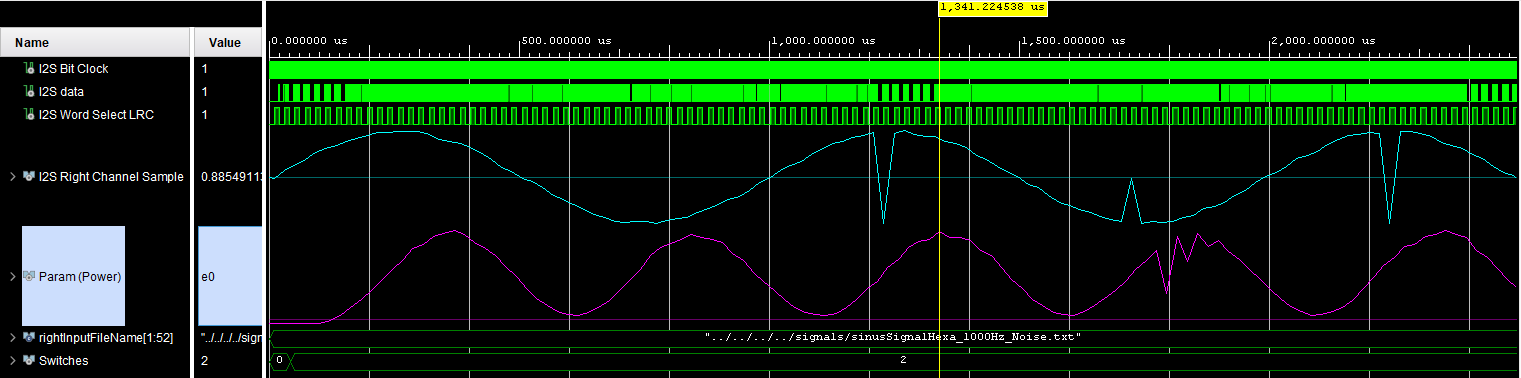
\includegraphics[width=\textwidth]{assets/chrono-m6-1000hz-sin-noisy.png}
    \caption{Signal sinusoïdal bruité à \SI{1}{\kilo\hertz}}
    \label{fig:chrono-m6-1000hz-sin-noisy}
  \end{subfigure}
  \begin{subfigure}{.496\linewidth}
    \centering
    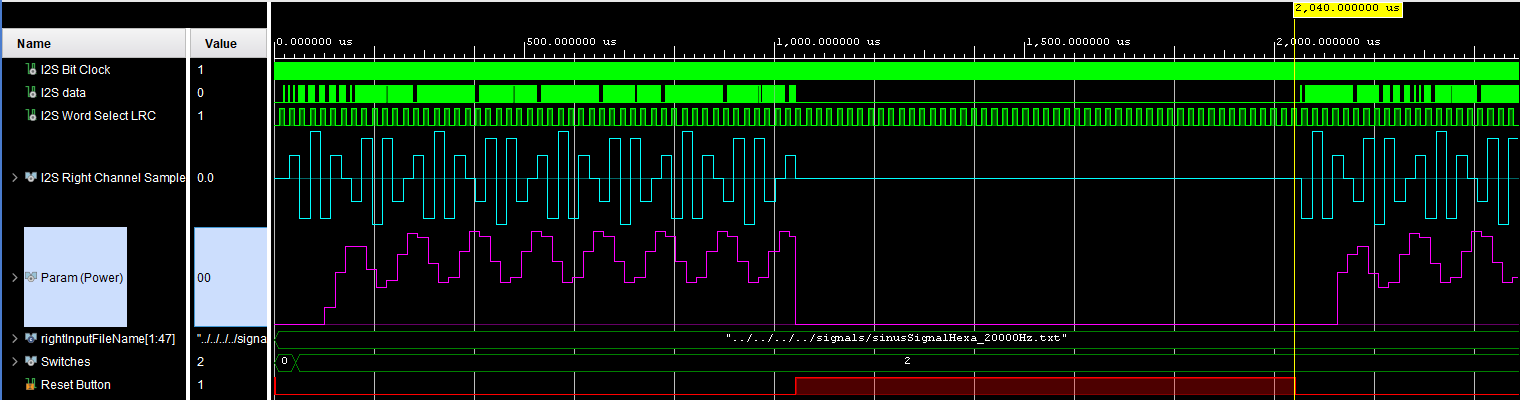
\includegraphics[width=\textwidth]{assets/chrono-m6-reset-and-20000hz.png}
    \caption{Post-réinitialisation et signal à \SI{20}{\kilo\hertz}}
    \label{fig:chrono-m6-reset-and-20000hz}
  \end{subfigure}
  \begin{subfigure}{.496\linewidth}
    \centering
    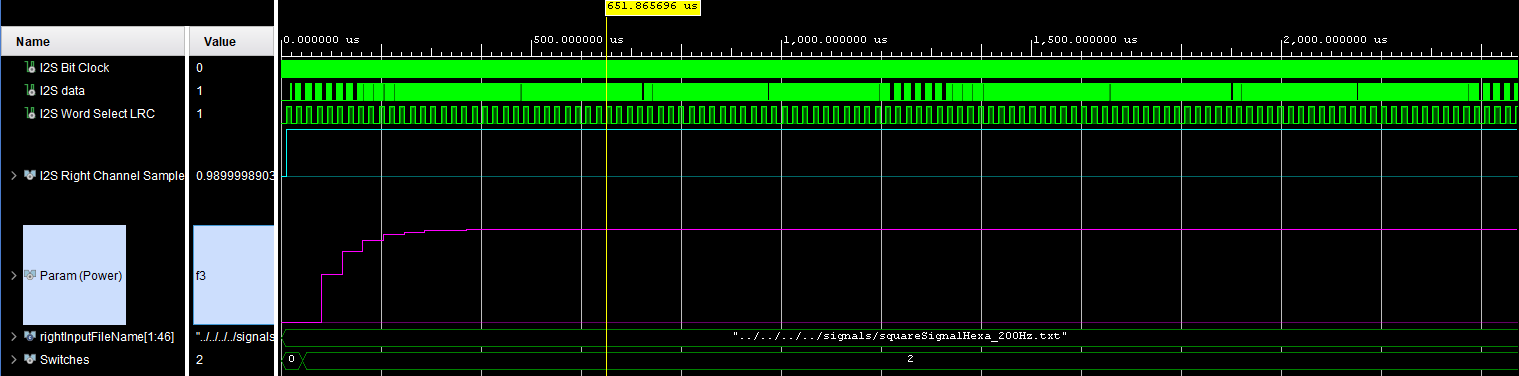
\includegraphics[width=\textwidth]{assets/chrono-m6-saturation-works.png}
    \caption{Saturation du module}
    \label{fig:chrono-m6-saturation-works}
  \end{subfigure}
  \begin{subfigure}{.496\linewidth}
    \centering
    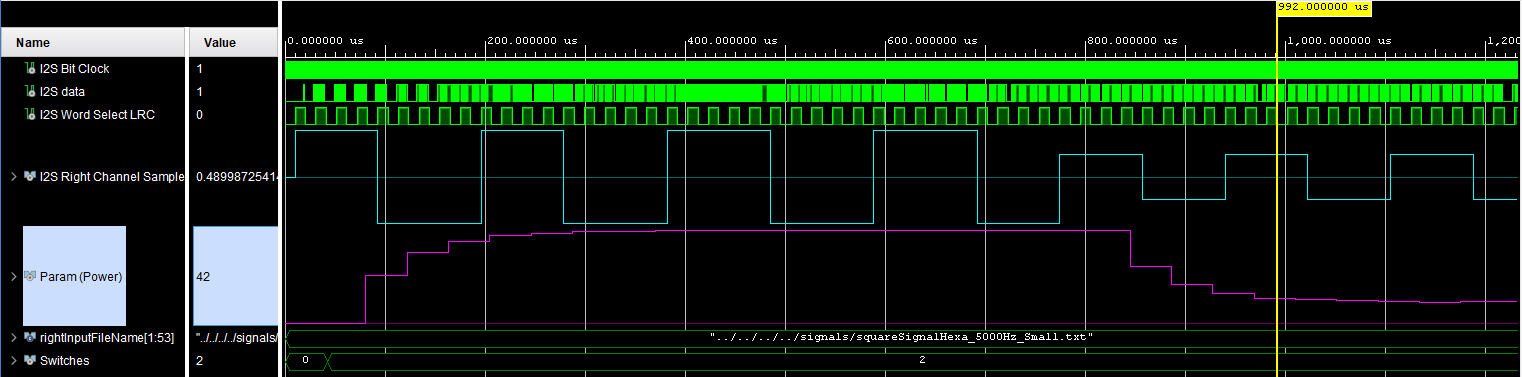
\includegraphics[width=\textwidth]{assets/chrono-m6-square-5000hz-2in1.png}
    \caption{Signal carré à 5000 Hz avec deux canaux}
    \label{fig:chrono-m6-square-5000hz-2in1}
  \end{subfigure}
  \caption{Chronographes du module M6 sous différentes conditions}
\end{figure}

% \quickfigure{Machine à états finis du module M6}{mef-m6}{}{assets/m6-mef-mermaid.pdf}

\todo{Schéma-bloc du système}

\subsection{Description du fonctionnement}

Le module M6 effectue une estimation de la puissance du signal audio en
appliquant un filtrage exponentiel à moyenne glissante sur les échantillons
entrants. Le calcul s'effectue à chaque front montant de l'horloge
\verb|i_bclk|, lorsque le signal \verb|i_en| est à 1. \\

À chaque activation, la puissance instantanée est calculée en élevant au
carré l'échantillon courant \verb|i_ech|. Cette nouvelle valeur est ensuite
ajoutée à l'historique de puissance, qui est préalablement réduite par un
facteur d'oubli de 31/32. Ce facteur assure que les résultats récents ont
plus de poids que les anciens, tout en limitant la croissance de la valeur
accumulée afin d'éviter un débordement (\emph{overflow}). \\

Le résultat final est stocké dans le registre \verb|oldest_power|. Pour
simplifier l'affichage ou l'utilisation de cette puissance, seuls les bits de
poids fort (\verb|oldest_power(46 downto 39)|) sont extraits et envoyés sur
la sortie \verb|o_param|. \\

% \todo{Description sommaire du fonctionnement}
\todo{Plan de vérification}

\todo{Validation via une simulation avec le banc de test fourni. Vous devez démontrer le
fonctionnement de vos modules au travers de simulations et expliquez en quoi vous
répondez aux spécifications. Faites bon usage des curseurs, formattage des données et
agrandissements pour appuyer vos propos.}
